\documentclass[fontsize=12pt, parskipp=full, paper=legal]{scrbook}
\usepackage{fontspec, xltxtra, xunicode}
\setromanfont[Scale=MatchLowercase,Mapping=tex-text]{Minion Pro}
\setsansfont[Scale=MatchLowercase,Mapping=tex-text]{DejaVu Sans}
\setmonofont[Scale=MatchLowercase]{DejaVu Sans Mono}

\usepackage[fixamsmath, centertags]{mathtools}
\usepackage{booktabs}

\usepackage{polyglossia}
\setdefaultlanguage{english}

\usepackage[cm]{fullpage}

\usepackage{color}
\usepackage{hyperref}
\hypersetup{colorlinks, urlcolor=blue, citecolor=blue}

\usepackage{verbments}
\DefineShortVerb{\¬}
\plset{
  language=scala,
  encoding=utf8,
  captionfont=\sffamily,
  style=tango,
  bgcolor=white,
  fvset={frame=lines}
}
%frame=lines, framerule=1pt, rulecolor=\color{black}
%baselinestretch=0.8},
%texcl=true,
%numbers=none,
%numbersep=5pt,
%belowcaptionskip=-8pt,

\usepackage{hyperref}
\hypersetup{
  linktocpage,
  colorlinks,
  citecolor=blue,
  filecolor=black,
  linkcolor=blue,
  urlcolor=blue
}

\usepackage{graphicx}
\everymath{\displaystyle}
\usepackage{enumerate}
\title{Basic programmig with Scala}
\author{M.C. Oscar Vargas Torres}
\begin{document}
\maketitle

\chapter{First steps}

\section{Your development environment for this course}
I recommend you to install these:
\begin{itemize}
\item Latest IntelliJ IDEA EAP version from here:\\
 \url{http://confluence.jetbrains.com/display/IDEADEV/IDEA+13+EAP}
\item Java 8 (the current java source code requires JDK 8) from here:\\
 \url{https://jdk8.java.net/download.html}
\item sbt (one of the Scala build tools available) following the
  instructions here:\\
 \url{http://www.scala-sbt.org/release/docs/Getting-Started/Setup.html}
\item git for your OS of choice.
\end{itemize}

\section{Running the code samples with sbt}
Once you can use sbt from the command line, start it, compile the code
samples and run ¬com.oscarvarto.HelloScala¬:
\begin{pyglist}[language=text]
$ pwd
/Users/oscarvarto/ScalaBasics
oscar-imac:ScalaBasics oscarvarto$ ls
README.md	build.sbt	doc		project		src
$ sbt
[info] Loading project definition from /Users/oscarvarto/ScalaBasics/project
[info] Updating {file:/Users/oscarvarto/ScalaBasics/project/}scalabasics-build...
[info] Resolving org.fusesource.jansi#jansi;1.4 ...
[info] Done updating.
[info] Set current project to scalaBasics (in build file:/Users/oscarvarto/ScalaBasics/)
> compile
[info] Updating {file:/Users/oscarvarto/ScalaBasics/}scalabasics...
[info] Resolving jline#jline;2.11 ...
[info] Done updating.
[info] Compiling 5 Scala sources and 4 Java sources to /Users/oscarvarto/ScalaBasics/target/scala-2.11.0-M8/classes...
[success] Total time: 7 s, completed Jan 25, 2014 5:30:24 AM
> run

Multiple main classes detected, select one to run:

 [1] com.oscarvarto.Arithmetics
 [2] com.oscarvarto.ControlFlowScala
 [3] com.oscarvarto.HelloJava
 [4] com.oscarvarto.ControlFlowJava
 [5] com.oscarvarto.ArithmeticsJava
 [6] com.oscarvarto.HelloVariablesJava
 [7] com.oscarvarto.fp.OptionExperiment
 [8] com.oscarvarto.HelloScala
 [9] com.oscarvarto.HelloVariables

Enter number: 8

[info] Running com.oscarvarto.HelloScala
Hello Scala
[success] Total time: 13 s, completed Jan 25, 2014 5:30:41 AM
>
\end{pyglist}

\emph{Note: The first time you run sbt you will have to wait while it
downloads some stuff.}

\section{Opening the source code in IntelliJ IDEA}
From the sbt prompt, type ¬gen-idea¬. You should see something like:
\begin{pyglist}[language=text]
> gen-idea
[info] Creating IDEA module for project 'scalaBasics' ...
[info] Resolving jline#jline;2.11 ...
[info] Excluding folder target
[info] Created /Users/oscarvarto/ScalaBasics/.idea/IdeaProject.iml
[info] Deleted existing library files
[info] Created /Users/oscarvarto/ScalaBasics/.idea
[info] Excluding folder /Users/oscarvarto/ScalaBasics/target
[info] Created /Users/oscarvarto/ScalaBasics/.idea_modules/scalaBasics.iml
[info] Created /Users/oscarvarto/ScalaBasics/.idea_modules/scalaBasics-build.iml
>
\end{pyglist}

Once you open the project in IntelliJ IDEA, you should be able to see
something like Figure~\ref{fig:scalaBasics-IntelliJ}.

\begin{figure}[h!]
  \centering
  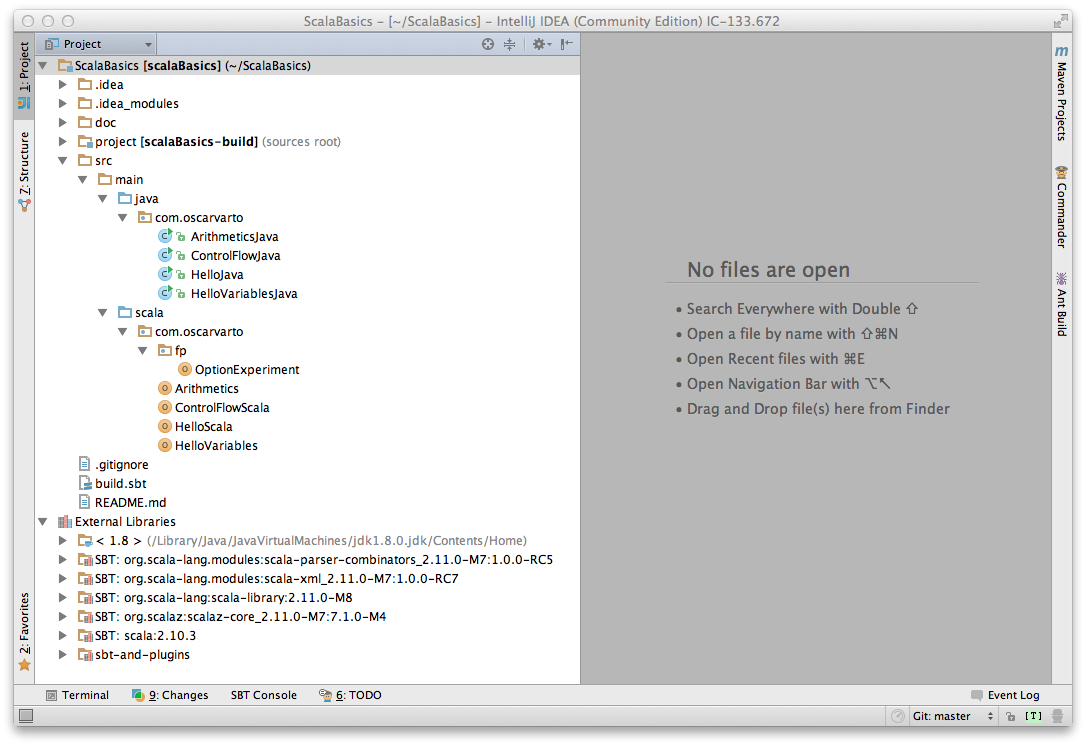
\includegraphics[scale=0.5]{figures/scalaBasicsIntelliJ.png}
  \caption{The ScalaBasics project opened in IntelliJ IDEA}
  \label{fig:scalaBasics-IntelliJ}
\end{figure}


\end{document}
%%% Local Variables:
%%% mode: latex
%%% TeX-master: t
%%% End:
